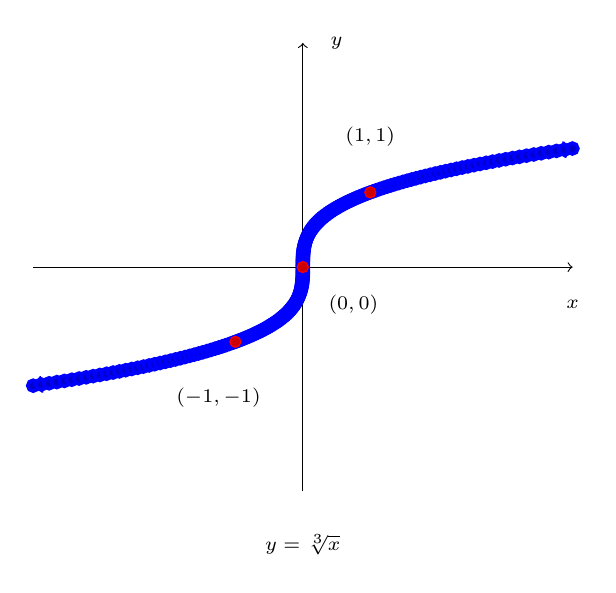
\begin{tikzpicture}
\begin{axis}[
  xmin=-4, xmax=4,
  ymin=-3, ymax=3,
  axis lines=middle,
  axis line style={->},
  ticks=none,
  clip=false
]
\node at (axis cs:4,-0.5){\scriptsize $x$};
\node at (axis cs:0.5,3){\scriptsize $y$};
\node at (axis cs:1,1.75){\scriptsize $(1,1)$};
\node at (axis cs:0.75,-0.5){\scriptsize $(0,0)$};
\node at (axis cs:-1.25,-1.75){\scriptsize $(-1,-1)$};

\addplot+[domain=-1.587:1.587, samples=200, smooth, line width=1.25pt, <->, variable=\t, parametric]
  ({\t^3},{\t});

\addplot+[only marks, mark=*, mark size=2pt] coordinates {(0,0) (1,1) (-1,-1)};

% Caption
\node at (rel axis cs:0.5,-0.12){\scriptsize $y=\sqrt[3]{x}$};
\end{axis}
\end{tikzpicture}